\section{Design the EKF time update step}

\subsection{Task 3}

To derive a discretized model from the continuous time model in equation (5), we can solve the differential equation and use the relation $exp(AΔt) \approx I + AΔt$ to obtain the discretized form. Here's the derivation:


Starting with the continuous-time model:
$\dot{q}(t) = \frac{1}{2}S(\omega_{k-1}+v_{k-1})q(t), \text{ for } t \in [t_{k-1}, t_k),$

Integrating both sides of the equation from $t_{k-1}$ to $t_k$, we have:
$\int_{t_{k-1}}^{t_k} \dot{q}(t) dt = \int_{t_{k-1}}^{t_k} \frac{1}{2}S(\omega_{k-1}+v_{k-1})q(t) dt.$

Applying the integral on the left side:
$q(t_k) - q(t_{k-1}) = \frac{1}{2}S(\omega_{k-1}+v_{k-1})\int_{t_{k-1}}^{t_k} q(t) dt.$

Using the relation $exp(AΔt) ≈ I + AΔt$, where $Δt = t_k - t_{k-1}$, we can approximate the integral term:
$\int_{t_{k-1}}^{t_k} q(t) dt \approx \Delta t \cdot q(t_{k-1}).$

Substituting this approximation back into the equation:
$q(t_k) - q(t_{k-1}) = \frac{1}{2}S(\omega_{k-1}+v_{k-1})\Delta t \cdot q(t_{k-1}).$

Rearranging the equation, we get:
$q(t_k) = (I + \frac{1}{2}\Delta t \cdot S(\omega_{k-1}+v_{k-1})) \cdot q(t_{k-1}).$

Comparing this with the discretized model $q_k = F(\omega_{k-1})q_{k-1} + G(\hat{q}_{k-1})v_{k-1},$ we can identify the expressions for $F$ and $G$ as follows:

$F(\omega_{k-1}) = I + \frac{1}{2}T\cdot S(\omega_{k-1}),$

$G(\hat{q}_{k-1}) = \frac{1}{2}T \cdot S(\hat{q}_{k-1}).$

Note: These derivation above is too weird that it reached the same result but the procedure is totally different.

\emph{Note2} :OK from combine slides and the report of Linkoping university, we can reach the same result.


\subsubsection{Reason for Discretize}

In the EKF, the prediction step involves propagating the state estimate and covariance from the previous time step to the current time step. This propagation is typically done using the continuous-time dynamic model, which can be linearized around the current state estimate. However, linearizing the model can introduce errors, especially for highly nonlinear systems.

To address this issue, the discretized model derived using the approximation techniques provides an alternative approach for the prediction step in the EKF. By discretizing the continuous-time dynamic model, we can directly apply it in the discrete-time domain without the need for linearization. This allows us to capture the nonlinearities of the system more accurately, especially when the nonlinearities are significant.

\subsection{Task 4}

If there are angular velocities, update the estimate and covariance as motion model, in function \texttt{tu\_qw}.

Once $ v_k $ is missing, use the same consideration as in homework 2, skip the update for current time and keep the state and covariance value as the latest update value.

\subsection{Task 5}

In the function \texttt{Task5\_filterTemple}, I applied the \texttt{tu\_qw} and \texttt{mu\_normalizeQ} functions for the sensor \emph{gyro}.

As observed and analysed before, \emph{gyro} is accurate for the angular velocities, but it can not accually get the absolute orientation.

So when I start from the phone face to left and stand on it left edge, it takes it as the intial flat state. In the process I shake it, it always has a bias, or to say, offset with the Goolge estimate figure.

\emph{Gyro} also has a feature that I will drift according to bias. So when I start with the phone on the table, shake it for some time and place it back, repeat this procedure twice, it clearly shows a dift process in figure \ref{fig:drift-process}:


\begin{figure}[H]
    \centering
    \begin{subfigure}[H]{0.3\textwidth}
        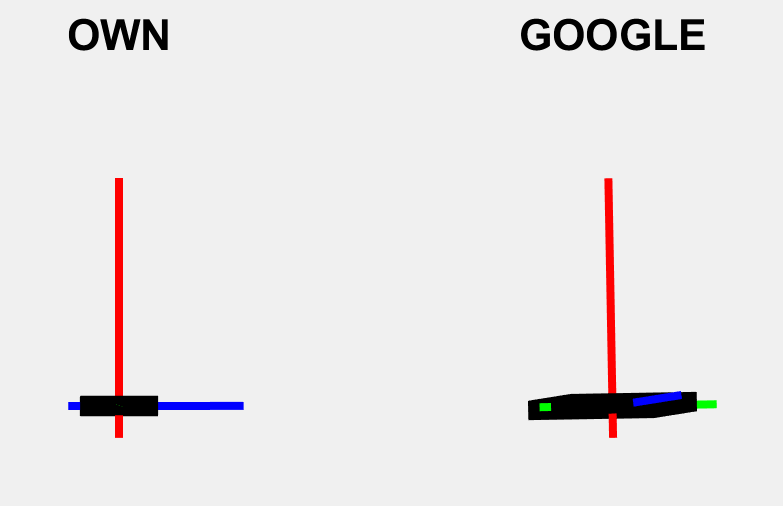
\includegraphics[width=\textwidth]{images/beginning.png}
        \caption{Begin}
        \label{fig:begin}
    \end{subfigure}
    \hfill
    \begin{subfigure}[H]{0.3\textwidth}
        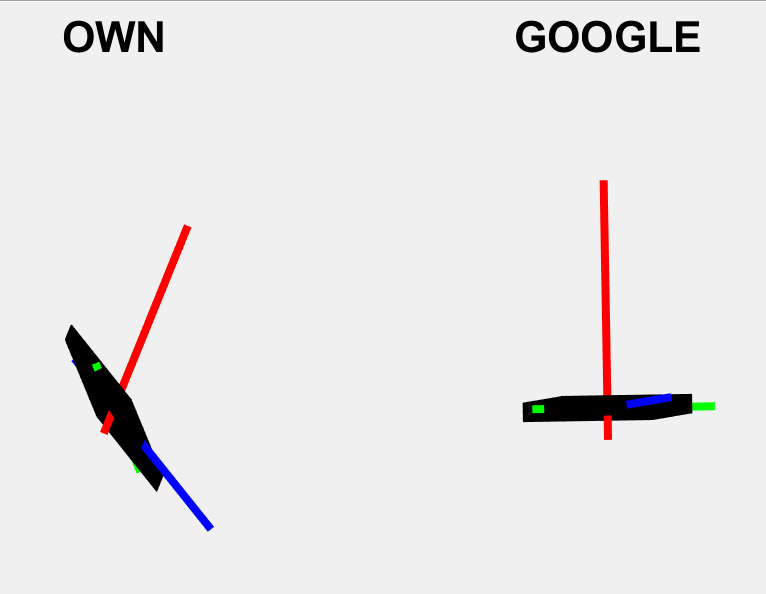
\includegraphics[width=\textwidth]{images/drift1.png}
        \caption{Firstshake}
        \label{fig:drift1}
    \end{subfigure}
    \hfill
    \begin{subfigure}[H]{0.3\textwidth}
        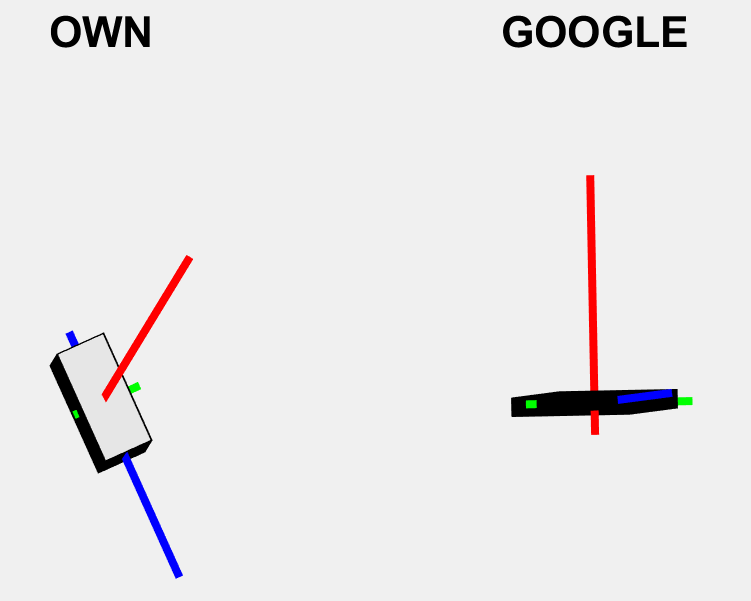
\includegraphics[width=\textwidth]{images/drift2.png}
        \caption{Secondshake}
        \label{fig:drift2}
    \end{subfigure}
    \caption{Drift Process}
    \label{fig:drift-process}
\end{figure}



